\documentclass[a4paper,14pt,twoside]{extarticle}
\usepackage[T2A]{fontenc}
\usepackage[utf8]{inputenc}
%\usepackage{cyrtimes}
\usepackage[english,russian]{babel}
\usepackage{indentfirst}
\usepackage{ccaption}

\captionnamefont{\sffamily}
\captiontitlefont{\sffamily}

\usepackage{tikz}
\usetikzlibrary{calc}
\usetikzlibrary{positioning}
\usetikzlibrary{mindmap}

\usepackage{background}
\usepackage{fancyhdr}
\pagestyle{fancy}
\renewcommand{\headrulewidth}{2pt}
\renewcommand{\footrulewidth}{0pt}
\fancyhead{}
\fancyhead[RO,LE]{\sffamily \slshape Отчёт по мониторингу проектов адаптации тротуаров}
\fancyhead[LO,RE]{\sffamily \thepage}
\fancyfoot{}

\title{Отчёт по мониторингу выполнения проектов адаптации
 тротуаров к велосипедному движению в г.~Минске
 в~2012—2013 годах}

\author{ОО «Минское велосипедное общество»}

\setlength{\parskip}{2pt}
\textheight23cm%

\renewcommand\emph[1]{\textbf{#1}}

\makeatletter%
\def\maketitle{%
\makeatletter%
\sffamily

\thispagestyle{empty}%
\SetBgAngle{180}
\SetBgPosition{0.9\textwidth,-1.1\textheight}
\SetBgContents{
\includegraphics[width=0.1\textwidth]{bike-wheel-clip-grey.pdf}}
\BgThispage
\begin{center}
\bfseries
\begin{tikzpicture}
    \draw [anchor=west] (0,0) node {
\includegraphics[width=0.5\textwidth]{bike-org-by-logo.pdf}};
    \draw [anchor=east] (0,0) node [align=right, xscale=1.3, yscale=1.6]
                                   {МИНСКОЕ\\
                                    ВЕЛОСИПЕДНОЕ\\
                                    ОБЩЕСТВО};
    \draw (0,-5) node [xscale=0.8,align=flush center,inner sep=5pt,text width=\textwidth]
                     {\Large \@title};
\end{tikzpicture}

\vfill

\begin{tikzpicture}
    \draw (0,0) node [xscale=0.8] {\large Минск, 2014};
\end{tikzpicture}

\end{center}
\newpage
\SetBgContents{}
\makeatother
}
\makeatother

\def\normalfont{\sffamily}

\begin{document}

\def\figurename{Фото}

\maketitle

%\section*{Введение}
%\subsection*{Введение}
Мониторинг проводился с целью оценить, насколько полно и качественно произведена адаптация тротуаров к велосипедному движению, проводившаяся в рамках Концепции обеспечения велосипедного движения. Все работы должны были быть полностью выполнены в 2012—2013~гг.

Обследования проводились 17—22 мая 2014 года.

\emph{Общее заключение}: ни один проект полностью не реализован.

\newpage
%\section*{Результаты обследования}%
\subsection*{Фрунзенский район}%
\emph{Участок}: нечётная сторона ул. Притыцкого, от просп. Пушкина до ул. Кунцевщина, чётная сторона ул. Притыцкого от ул. Кунцевщина до Каменногорской ул.

\emph{Понижение бортовых камней}: Бортовые камни не понижены или понижены не в соответствии с проектом.

\emph{Разметка, знаки}: есть

\emph{Примечание}: выполнено понижение бортовых камней на противоположной стороне улицы.

\emph{Заключение}: по-видимому, из-за несогласованности работы участников проекта, было выполнено понижение бортовых камней на чётной стороне ул. Притыцкого (от просп. Пушкина до ул. Кунцевщина) не в соответствии с проектом, после чего нанесена разметка и установлены знаки в соответствии с проектом по нечётной стороне. Требуется выполнение понижения бортов по нечётной стороне. Объект не готов.

\emph{Дополнительно}: при проектировании и строительстве комплекса\linebreak «Green City» (между Нёманской ул. и ул. Кунцевщина) не было учтено наличие велодорожки: на проезде к комплексу отсутствует велопереезд (фото 1). Высота бортового камня на проезде не соответствует нормативам (фото 2), по которым перепада высот быть не должно.

\begin{figure}[hb!]
    %\begin{minipage}{0.8\textwidth}
        \centering
        %\hrule~\\[1ex]
        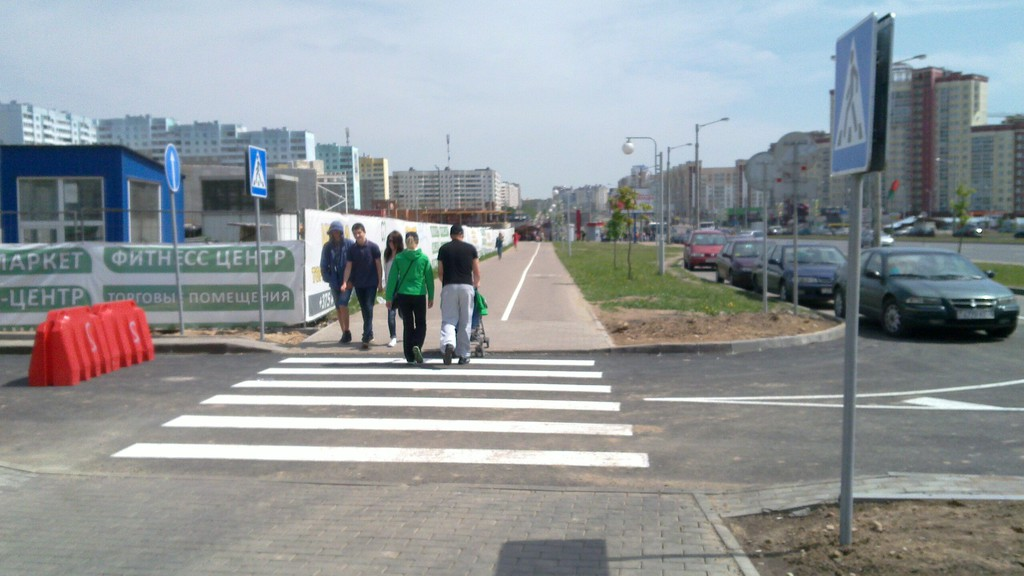
\includegraphics[width=0.9\textwidth]{Pictures/1000000000000A00000005A0BEC879E2.jpg}
        \caption{Проезд к комплексу «Green City». Отсутствует велопереезд}
        %\hrule
    %\end{minipage}
\end{figure}

\begin{figure}[h!]
        \centering
        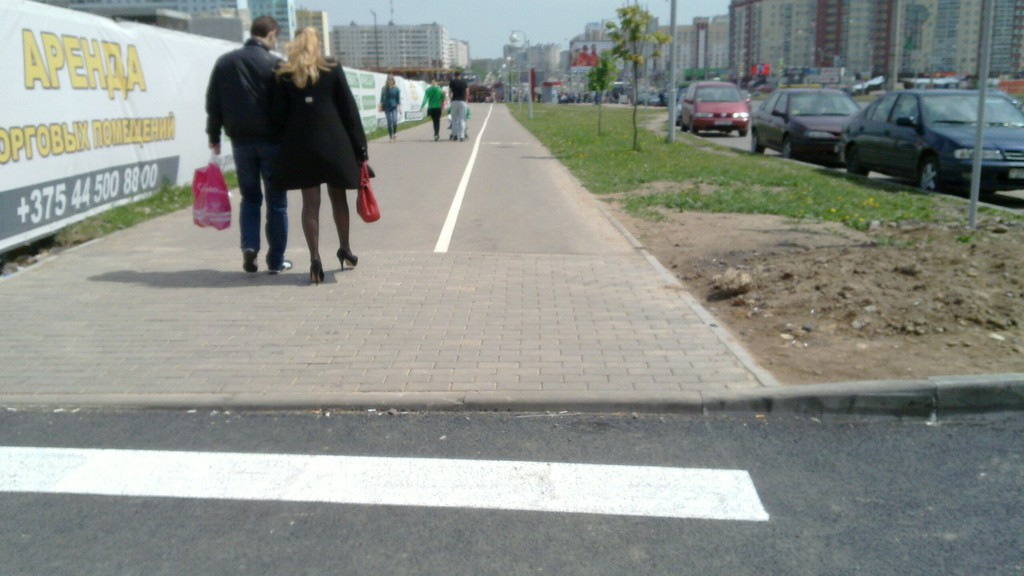
\includegraphics[width=\textwidth]{Pictures/1000000000000A00000005A062A3E4CA.jpg}
        \caption{Проезд к «Green City». Высота борта не нулевая}
\end{figure}

\begin{figure}[h!]
        \centering
        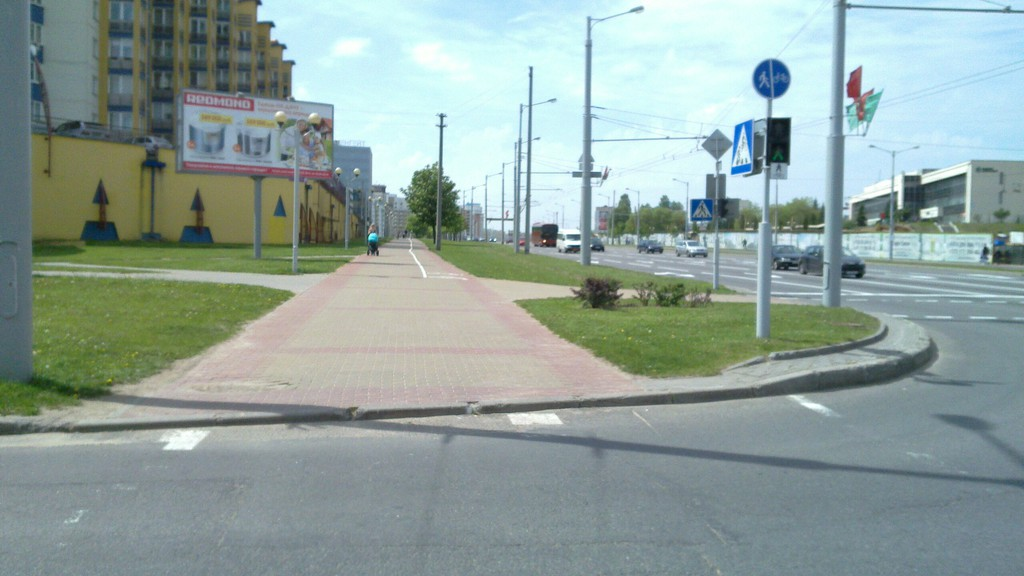
\includegraphics[width=\textwidth]{Pictures/1000000000000A00000005A028520F90.jpg}
        \caption{ул. Притыцкого. Бордюры по данной стороне улицы не понижались}
\end{figure}

\clearpage
\newpage

\subsection*{Центральный район}
\emph{Участок}: проспект Машерова, чётная сторона от ул. Кропоткина до ул. Тимирязева

\emph{Понижение бортовых камней}: Бортовые камни не понижены или понижены не в соответствии с проектом: пересечения с ул. Грибоедова, Гвардейской ул., Старовиленским трактом. При замене покрытия на ул. Тимирязева не выдержаны нормативы по высоте бортовых камней на переходах.

\emph{Разметка, знаки}: отсутствуют.

\emph{Заключение}: понижение бортовых камней выполнено не полностью, разметка и знаки отсутствуют, объект не готов.

\begin{figure}[hb!]
        \centering
        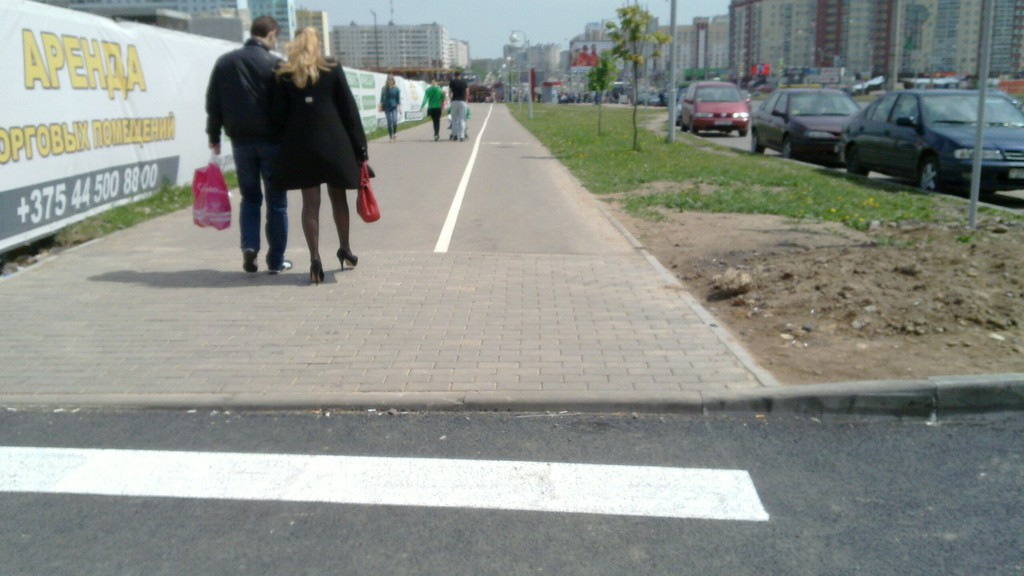
\includegraphics[width=\textwidth]{Pictures/1000000000000A00000005A062A3E4CA.jpg}
        \caption{Проезд к «Green City». Высота борта не нулевая}
\end{figure}

\begin{figure}[h!]
    \centering
    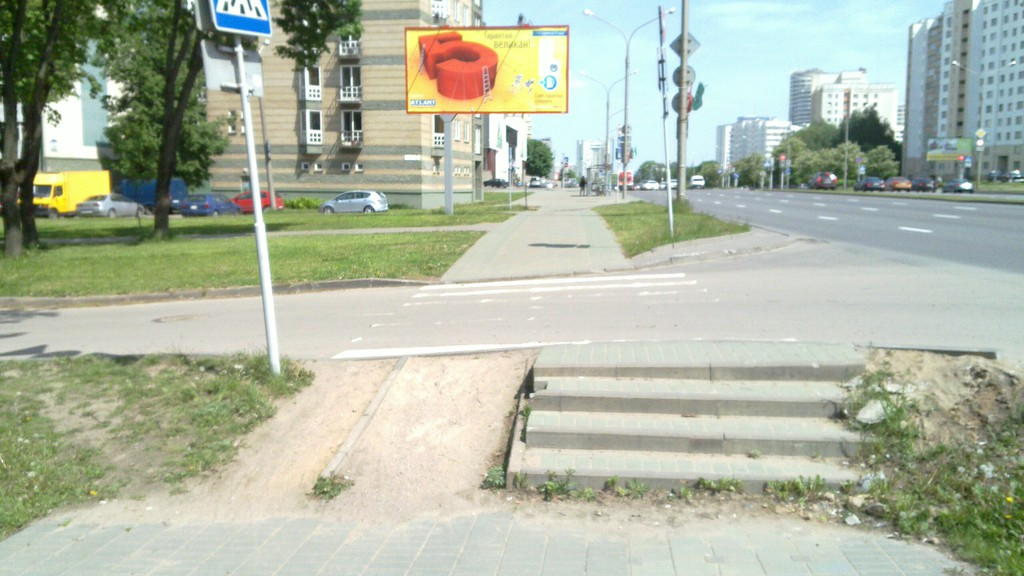
\includegraphics[width=\textwidth]{Pictures/1000000000000A00000005A0B4C7E123.jpg}
    \caption{ул. Грибоедова}
\end{figure}

\begin{figure}[h!]
    \centering
    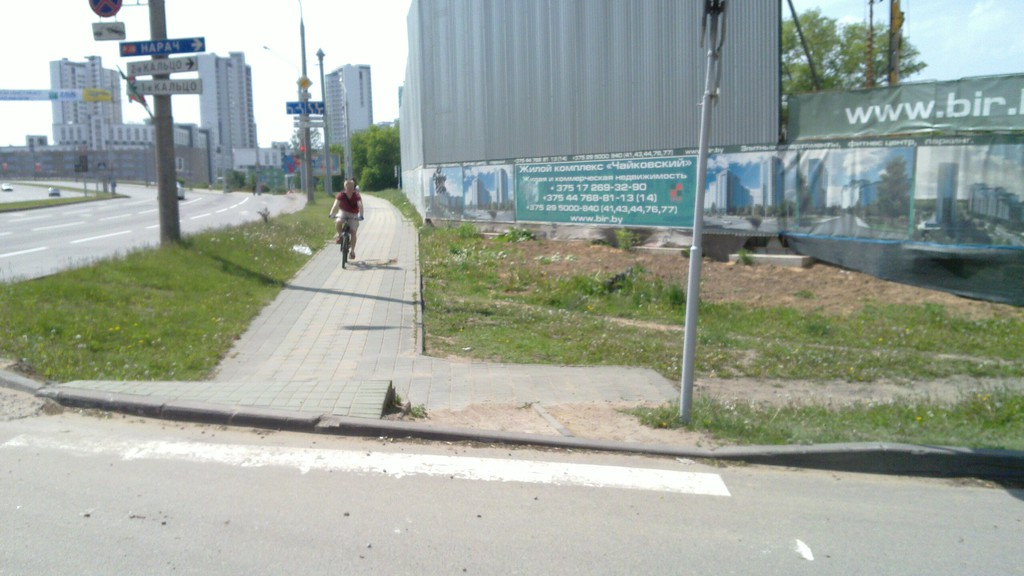
\includegraphics[width=\textwidth]{Pictures/1000000000000A00000005A0A7B34678.jpg}
    \caption{ул. Грибоедова}
\end{figure}

\begin{figure}[h!]
    \centering
    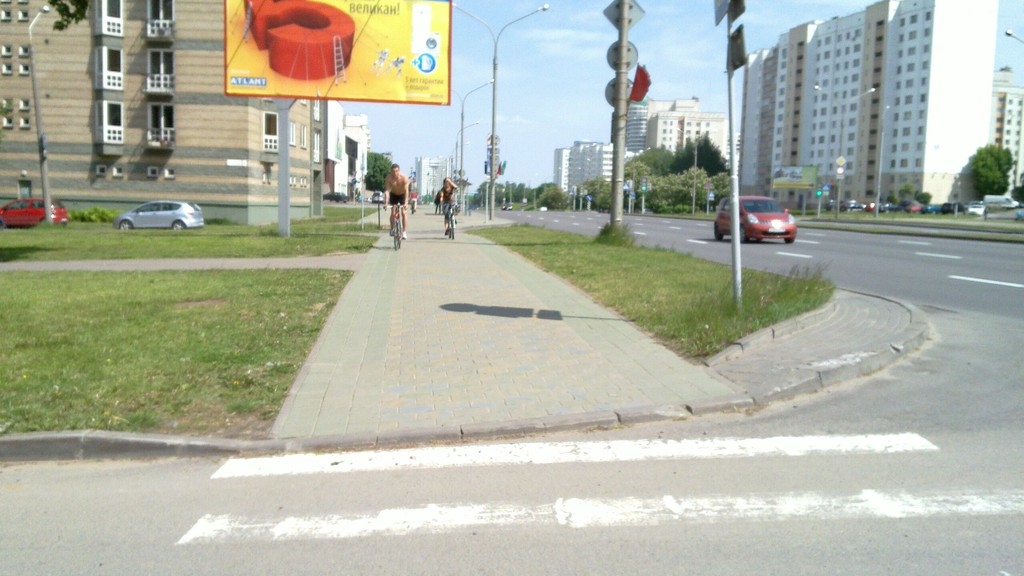
\includegraphics[width=\textwidth]{Pictures/1000000000000A00000005A04FA06081.jpg}
    \caption{ул. Грибоедова}
\end{figure}

\begin{figure}[h!]
    \centering
    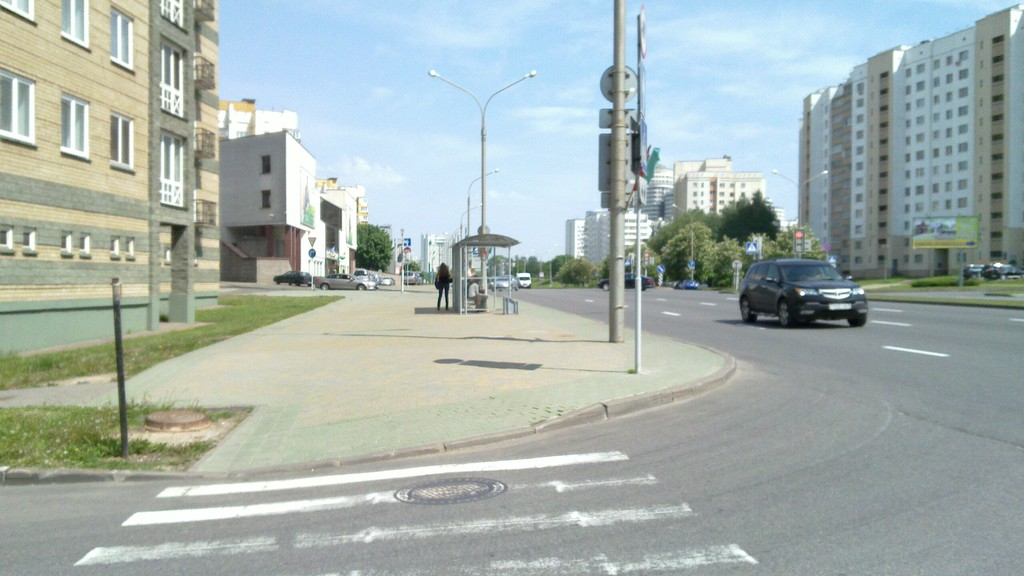
\includegraphics[width=\textwidth]{Pictures/1000000000000A00000005A0247D0B4C.jpg}
    \caption{ул. Грибоедова}
\end{figure}

\begin{figure}[h!]
    \centering
    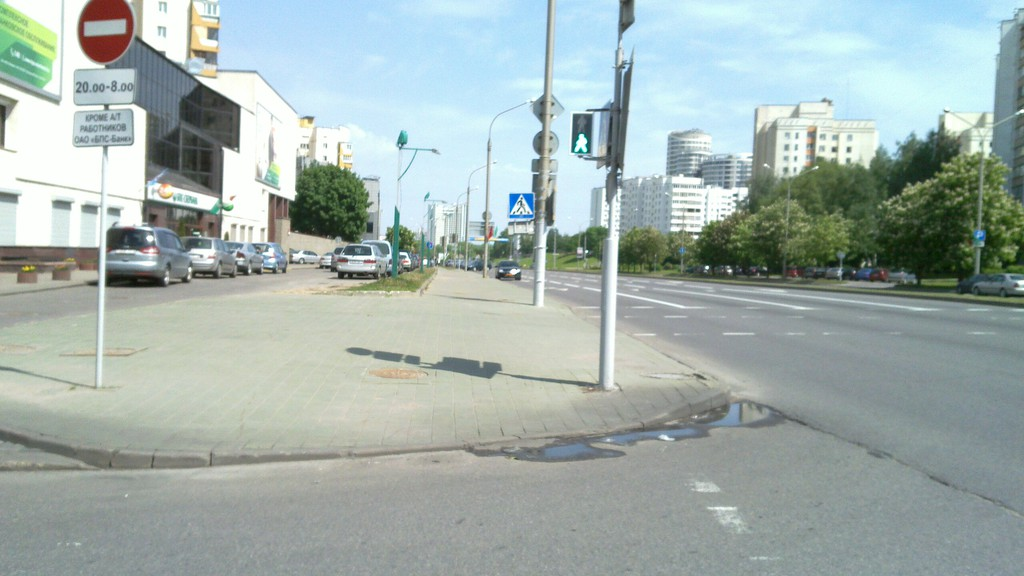
\includegraphics[width=\textwidth]{Pictures/1000000000000A00000005A069334A79.jpg}
    \caption{Гвардейская ул.}
\end{figure}

\begin{figure}[h!]
    \centering
    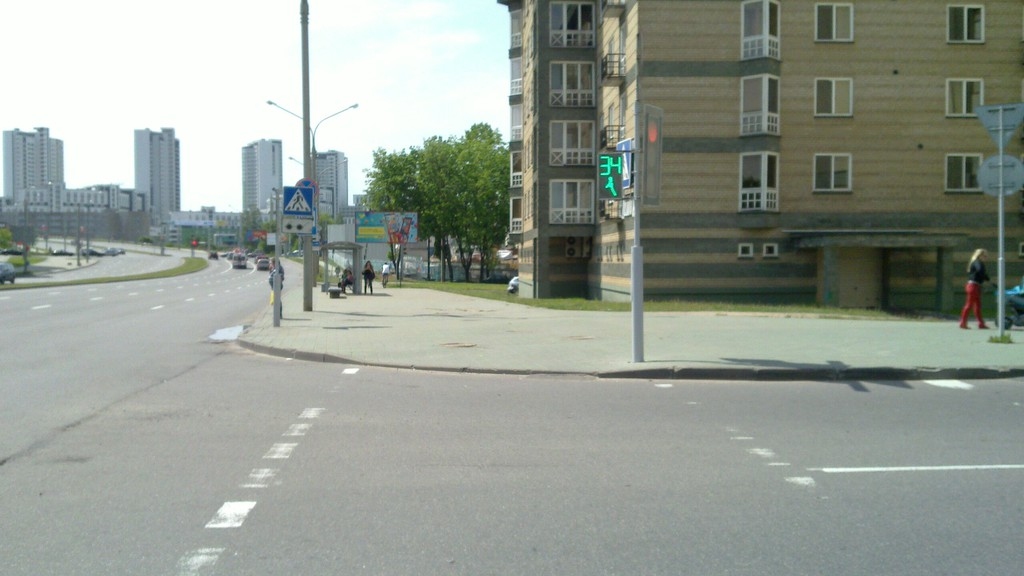
\includegraphics[width=\textwidth]{Pictures/1000000000000A00000005A02C4E92DF.jpg}
    \caption{Гвардейская ул.}
\end{figure}

\begin{figure}[h!]
    \centering
    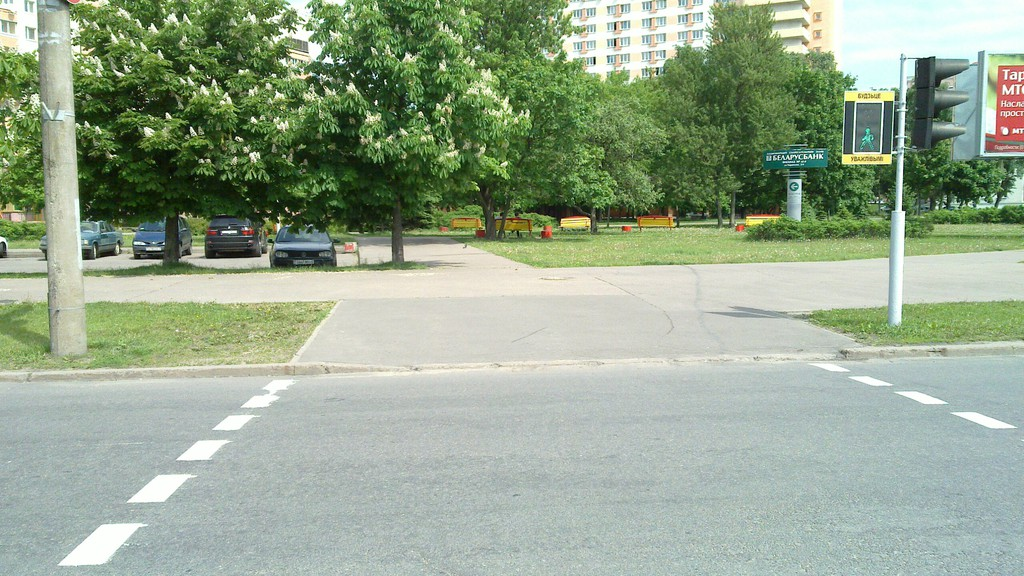
\includegraphics[width=\textwidth]{Pictures/1000000000000A00000005A0C349AD32.jpg}
    \caption{Старовиленский тракт}
\end{figure}

\begin{figure}[h!]
    \centering
    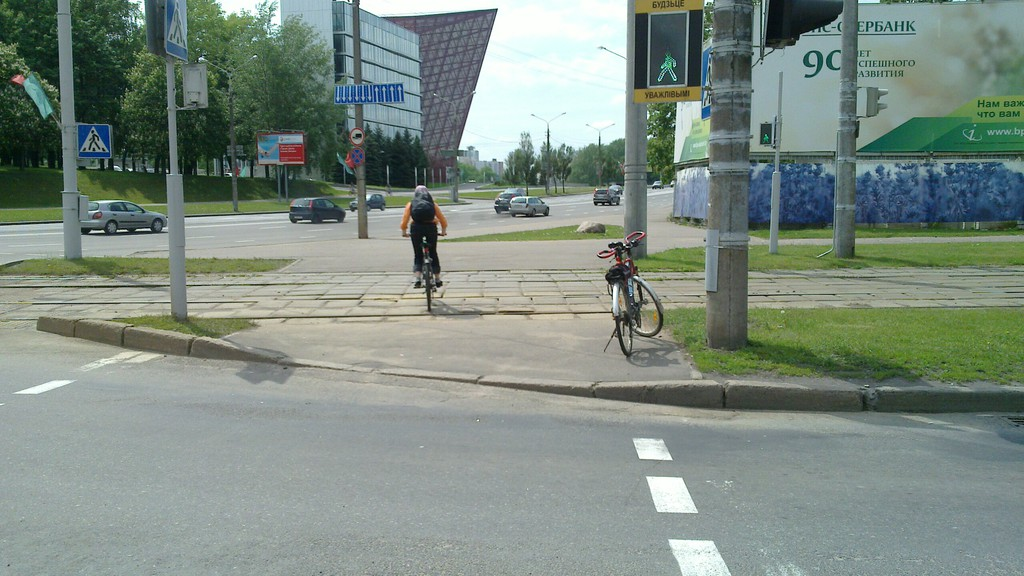
\includegraphics[width=\textwidth]{Pictures/1000000000000A00000005A0DC8DFB74.jpg}
    \caption{Старовиленский тракт}
\end{figure}

\clearpage
\newpage

\subsection*{Советский район}
\emph{Участок}: проспект Машерова и ул. Козлова, от ул. Кропоткина до Берестянской ул.

\emph{Понижение бортовых камней}: Во время реконструкции трамвайной остановки и путей на перекрёстке с Красной ул. не учтена проектируемая велодорожка (установлены ограждения). На пересечении с Берестянской ул. после обустройства автомобильной парковки высота бортовых камней на пешеходном переходе не соответствует нормативам. Не понижены: заезд к офису «Приорбанка» (Машерова, 40), Красная ул..

\emph{Разметка, знаки}: отсутствуют.

\emph{Заключение}: понижение бортовых камней выполнено не полностью, разметка и знаки отсутствуют, объект не готов.

\begin{figure}[h!]
    \centering
    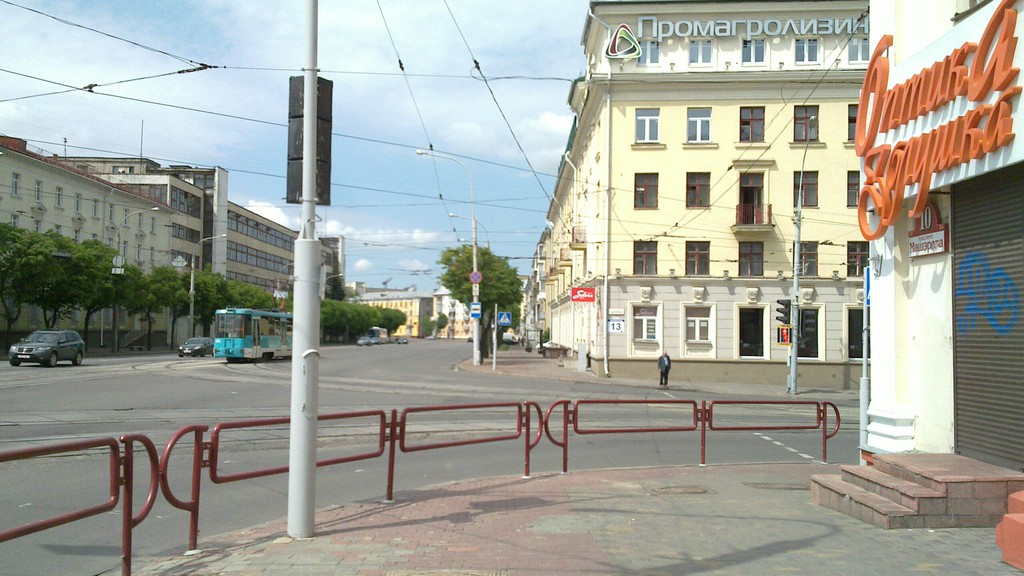
\includegraphics[width=\textwidth]{Pictures/1000000000000A00000005A061034552.jpg}
    \caption{Красная ул.}
\end{figure}

\begin{figure}[h!]
    \centering
    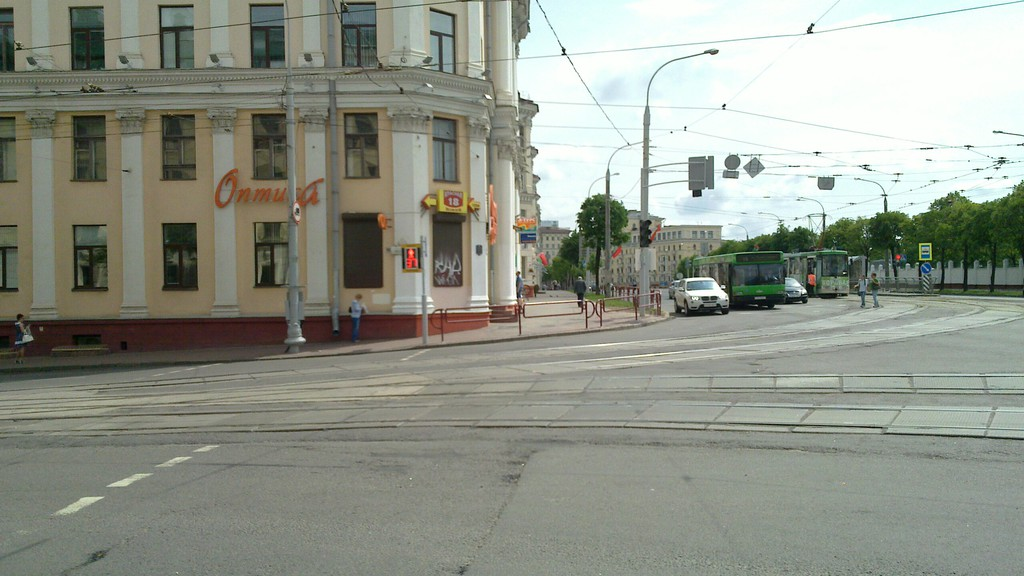
\includegraphics[width=\textwidth]{Pictures/1000000000000A00000005A0862511C0.jpg}
    \caption{Красная ул.}
\end{figure}

\begin{figure}[h!]
    \centering
    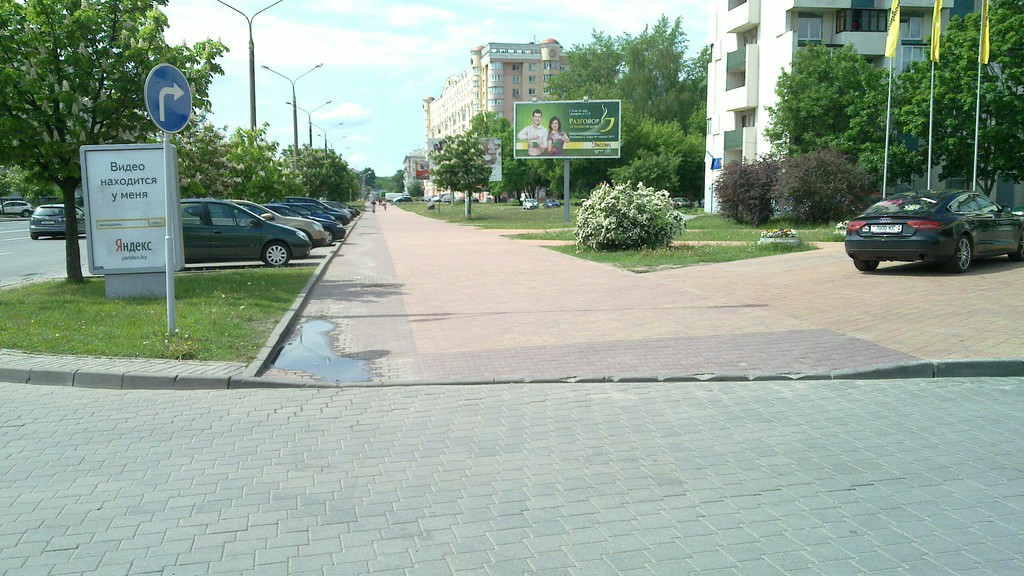
\includegraphics[width=\textwidth]{Pictures/1000000000000A00000005A038E55DC7.jpg}
    \caption{Проезд к Приорбанку}
\end{figure}

\begin{figure}[h!]
    \centering
    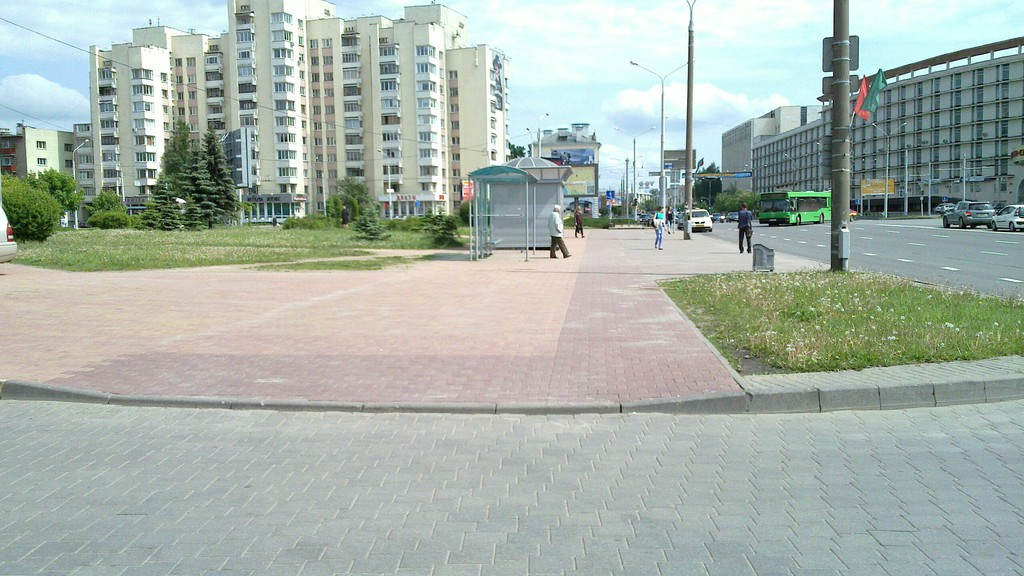
\includegraphics[width=\textwidth]{Pictures/1000000000000A00000005A0FD36DCD5.jpg}
    \caption{Проезд к Приорбанку}
\end{figure}

\begin{figure}[h!]
    \centering
    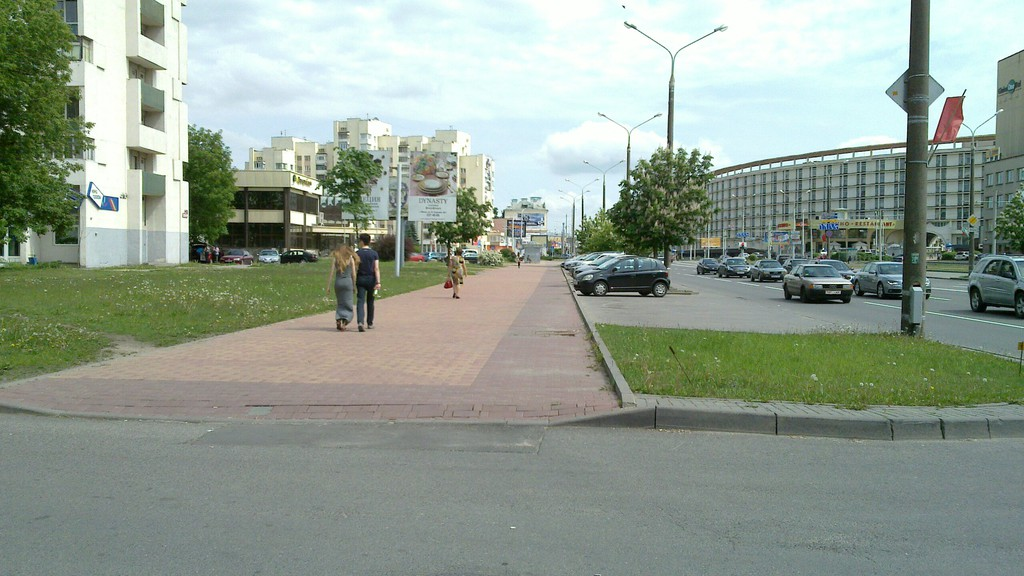
\includegraphics[width=\textwidth]{Pictures/1000000000000A00000005A0A8601281.jpg}
    \caption{Проезд к дому 42. Пониженный участок не доходит до края тротуара}
\end{figure}

\begin{figure}[h!]
    \centering
    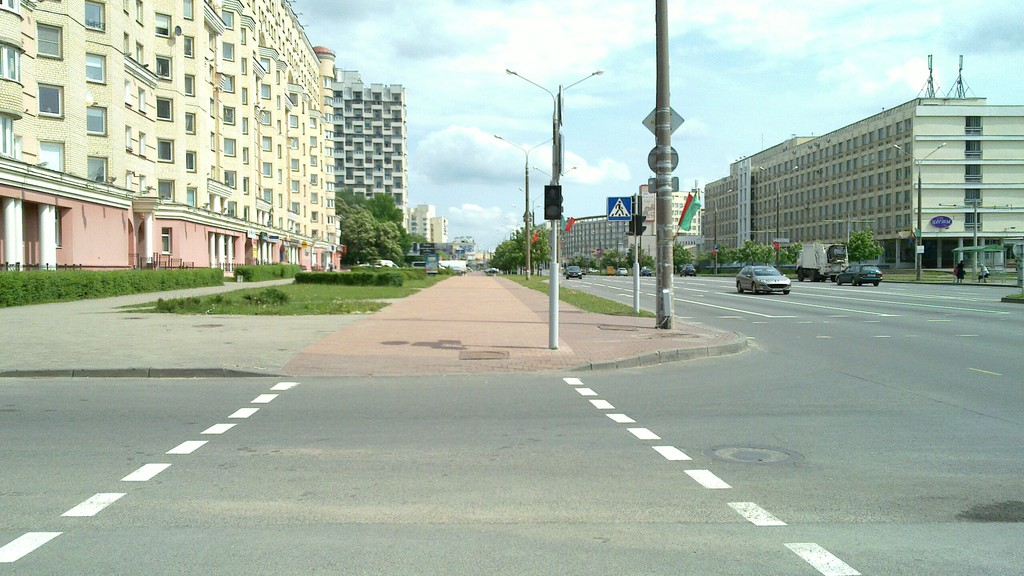
\includegraphics[width=\textwidth]{Pictures/1000000000000A00000005A0993F6107.jpg}
    \caption{ул. Кропоткина}
\end{figure}

\begin{figure}[h!]
    \centering
    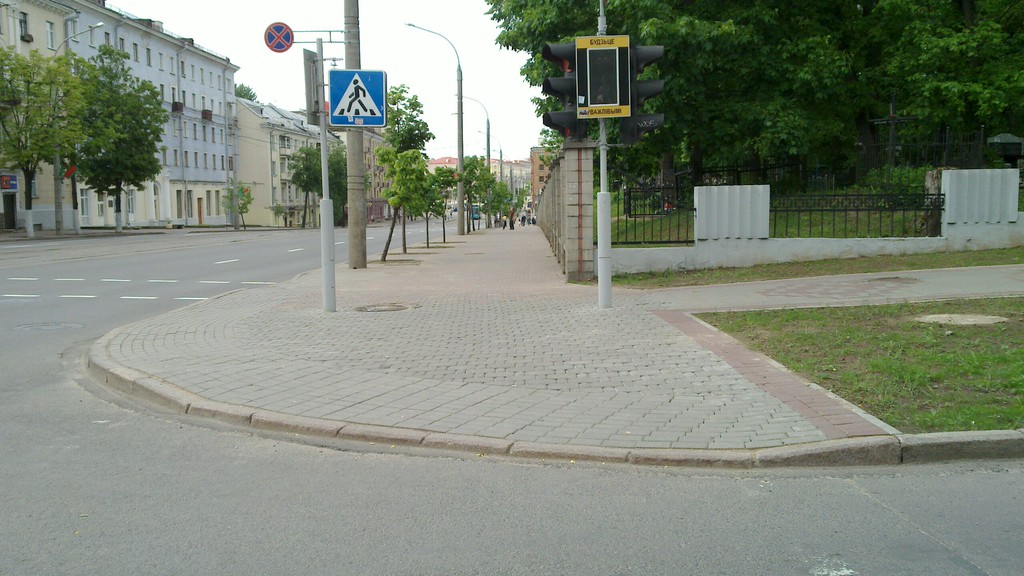
\includegraphics[width=\textwidth]{Pictures/1000000000000A00000005A0A1C3E05B.jpg}
    \caption{Берестянская ул.}
\end{figure}

\clearpage
\newpage

\emph{Участок}: ул. Кропоткина (от ул. Веры Хоружей) — ул. Карастояновой — ул. Некрасова (до перехода в районе ул. Неждановой)

\emph{Понижение бортовых камней}:
Бортовые камни понижены во всех местах, предусмотренных проектом. В случаях, когда высота бордюра была небольшой, обустроены асфальтовые пандусы, но с заглублением на проезжей части, что увеличивает их прочность (не будут повреждены уборочной техникой). Однако в некоторых местах зона понижения не доходит до границ тротуара. Несмотря на это, низкая интенсивность движения велосипедистов и пешеходов позволяет пользоваться веломаршрутом и в этом случае.

\emph{Разметка, знаки}: отсутствуют.

\emph{Заключение}: в части понижения бортовых камней работу можно считать выполненной, следует обратить внимание при выполнении будущих проектов на имеющиеся замечания. Требуется установка знаков, нанесение разметки.

\begin{figure}[h!]
    \centering
    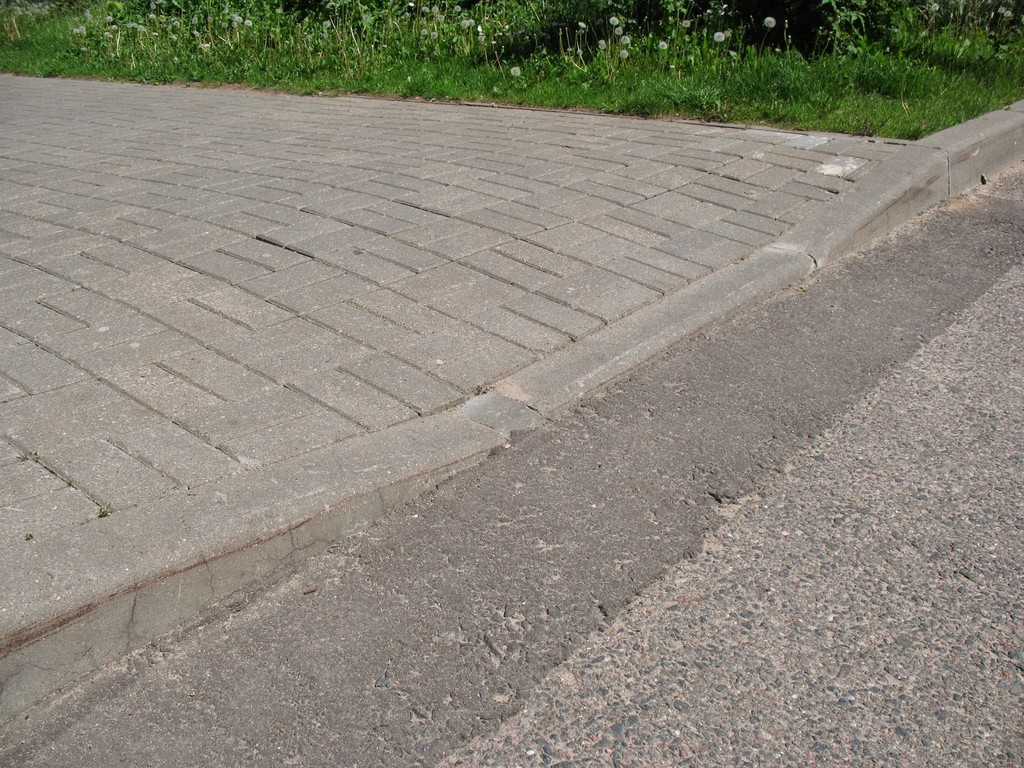
\includegraphics[width=\textwidth]{Pictures/100000000000080000000600A54E4DB9.jpg}
    \caption{Зона понижения бордюра не доходит до границ тротуара}
\end{figure}

\clearpage
\newpage

\subsection*{Первомайский район}
\emph{Участок}: проспект Независимости, чётная сторона от Филимонова до ул. Героев 120-й дивизии.

\emph{Понижение бортовых камней}: Понижение бортов на пересечении с ул. Руссиянова выполнено некачественно и требует переделки.

\emph{Разметка, знаки}: нет.

\emph{Примечание}: Велодорожка не учтена в проектах организации движения в районе нового квартала «Маяк Минска». На участке Руссиянова–Стариновская по маршруту велодорожки находится большое количество объектов притяжения пешеходов, которых не было на момент проектирования (павильоны Белсоюзпечати и другие).

\emph{Заключение}: Работы по проекту практически не выполнялись. Объект не готов. Требуется пересмотр и корректировка проекта для увязки с изменениями на местности и другими проектами организации движения.

\begin{figure}[h!]
    \centering
    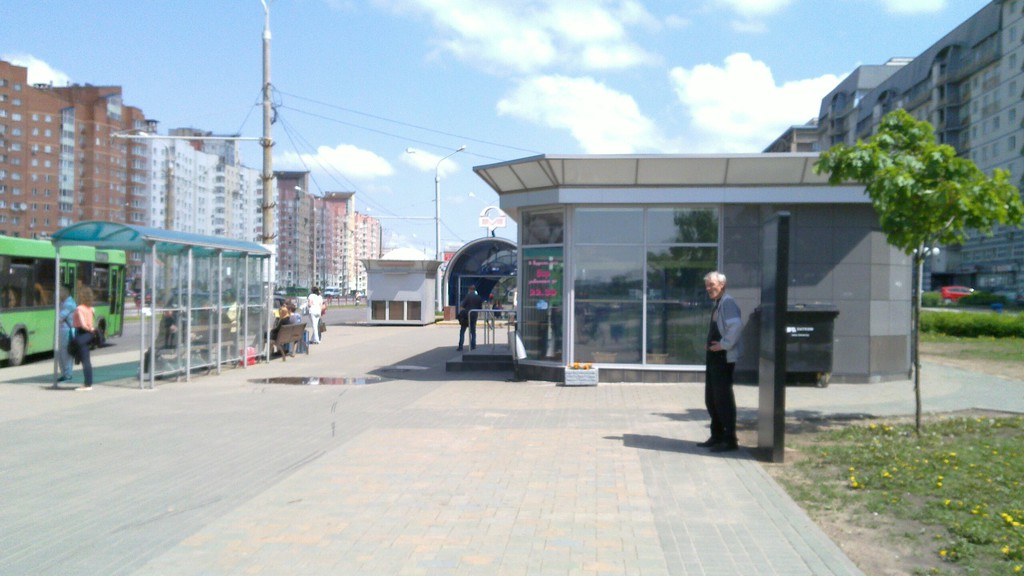
\includegraphics[width=\textwidth]{Pictures/1000000000000A00000005A0A7383363.jpg}
    \caption{Павильон Белсоюзпечати}
\end{figure}

\begin{figure}[h!]
    \centering
    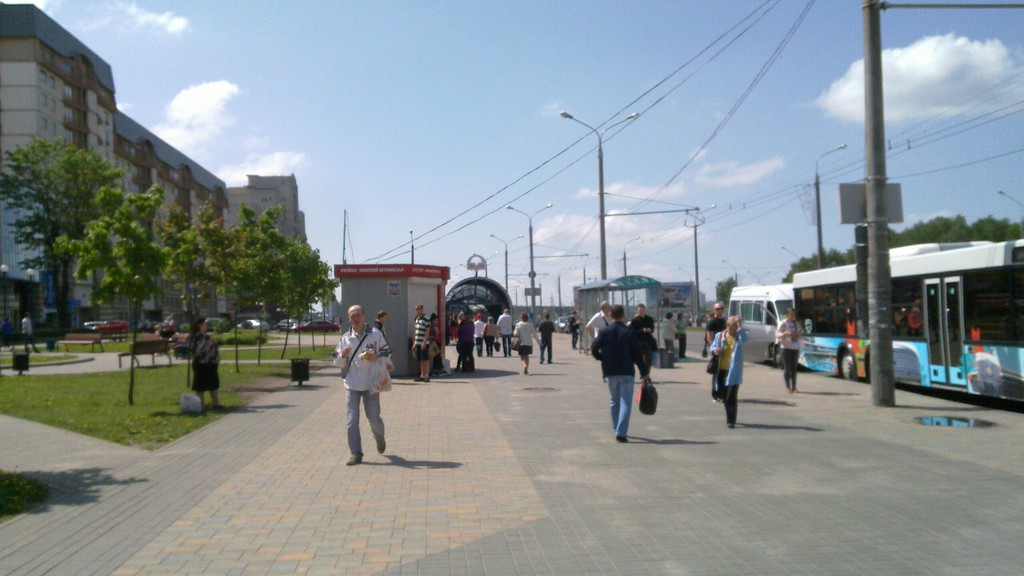
\includegraphics[width=\textwidth]{Pictures/1000000000000A00000005A0C142740A.jpg}
    \caption{Киоск «Минсктранс» и остановка ОТ}
\end{figure}

\begin{figure}[h!]
    \centering
    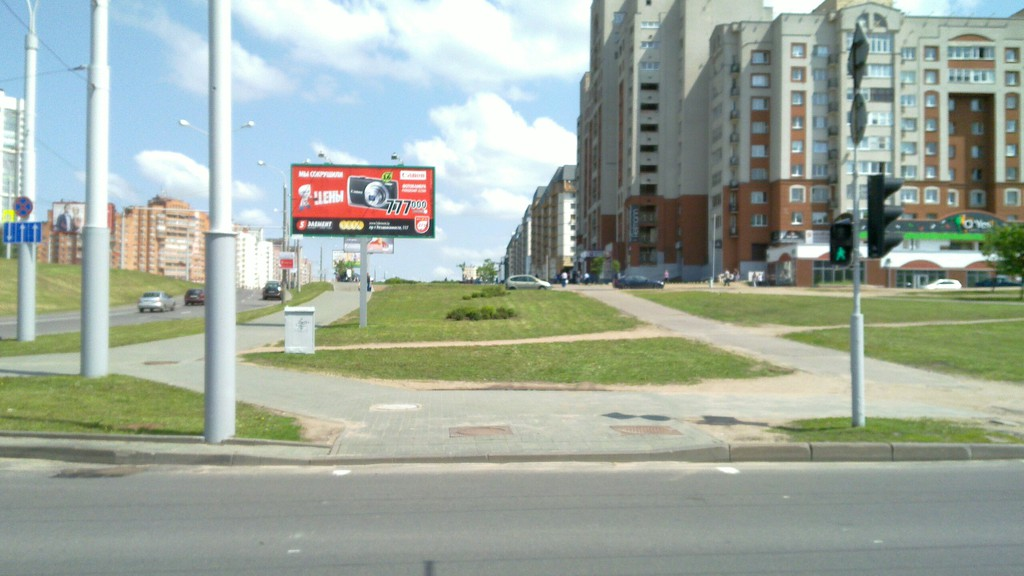
\includegraphics[width=\textwidth]{Pictures/1000000000000A00000005A05FA4F502.jpg}
    \caption{ул. Руссиянова. Бортовой камень понижен не до конца}
\end{figure}

\begin{figure}[h!]
    \centering
    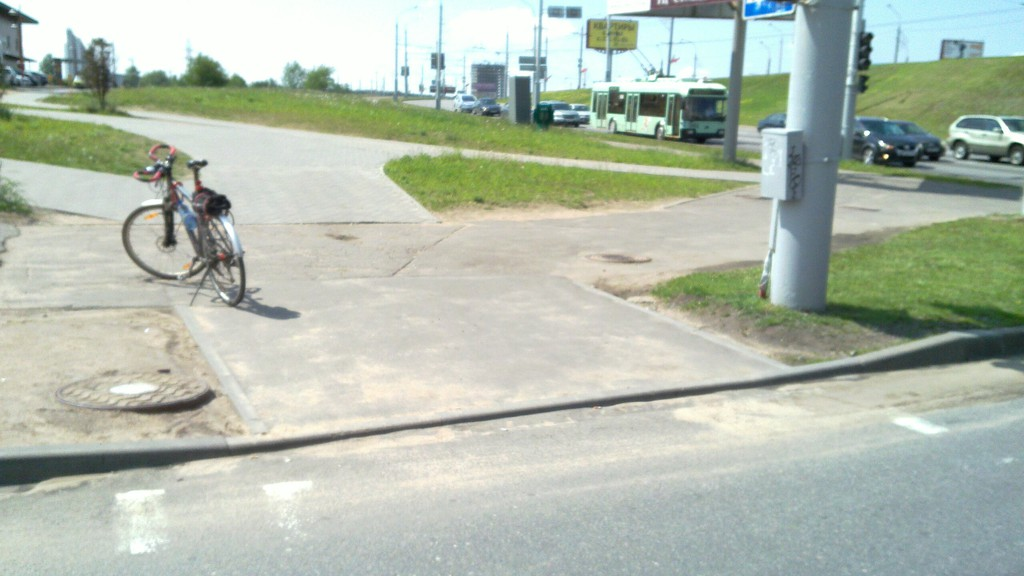
\includegraphics[width=\textwidth]{Pictures/1000000000000A00000005A0831C2317.jpg}
    \caption{ул. Руссиянова}
\end{figure}

\begin{figure}[h!]
    \centering
    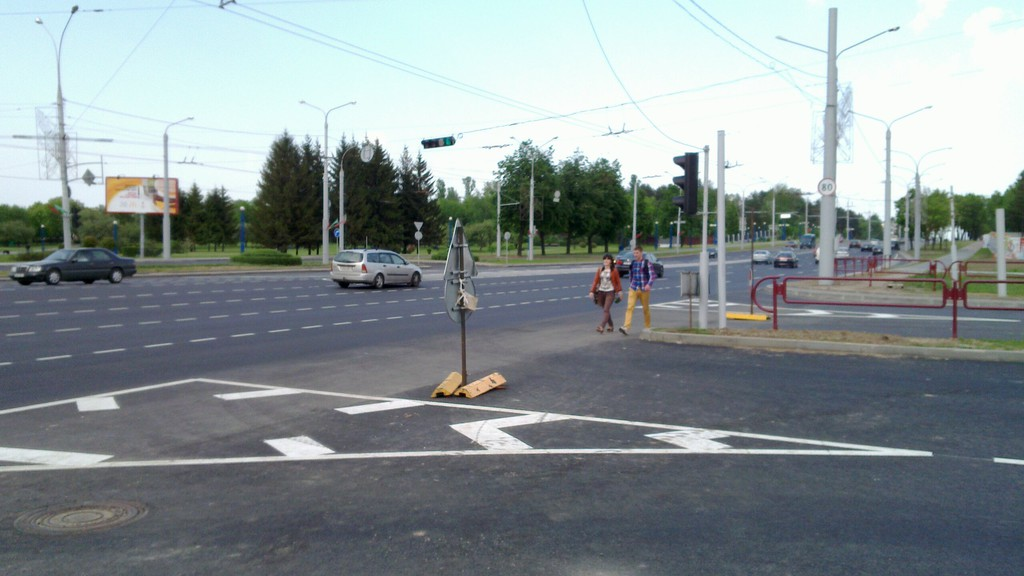
\includegraphics[width=\textwidth]{Pictures/1000000000000A00000005A085C46430.jpg}
    \caption{Новая улица (Кирилла Туровского). Пешеходы и велосипедисты из-за удалённости пешеходного перехода пересекают дорогу в запрещённом месте, несмотря на ограждение.}
\end{figure}

\begin{figure}[h!]
    \centering
    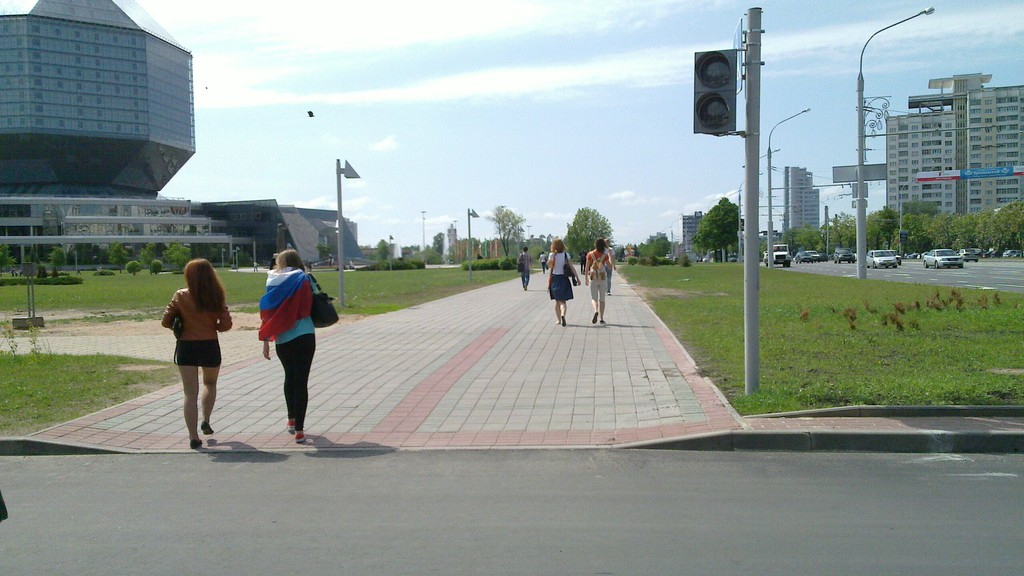
\includegraphics[width=\textwidth]{Pictures/1000000000000A00000005A02D5A121F.jpg}
    \caption{Новая улица, «Маяк Минска». Пониженная часть не доходит до края тротуара}
\end{figure}

\begin{figure}[h!]
    \centering
    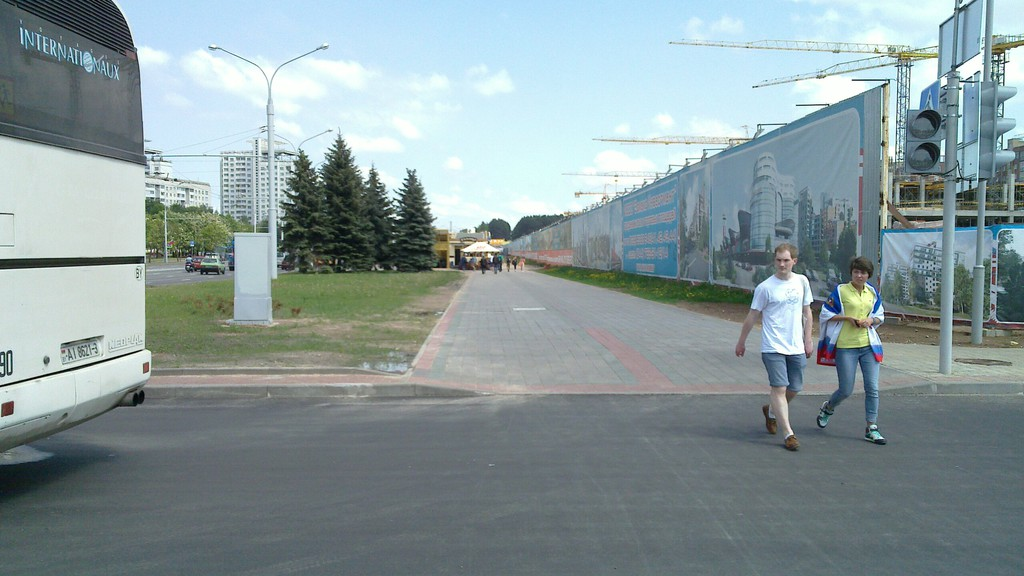
\includegraphics[width=\textwidth]{Pictures/1000000000000A00000005A0644D364B.jpg}
    \caption{Новая улица, «Маяк Минска». Пониженная часть не доходит до края тротуара}
\end{figure}

\clearpage
\newpage

\subsection*{Партизанский район}
\emph{Участок}: ул. Захарова от Первомайской ул. до Андреевской ул., Андреевская ул. от Захарова до Пулихова, ул. Пулихова от Андреевской до Первомайской (коммутирующая велодорожка, связывающая район с магистральной велодорожкой вдоль Свислочи).

\emph{Понижение бортовых камней}: Не понижены бортовые камни на пересечениях с заездами на хладокомбинат, к дому №50В. В ходе реконструкции подстанции скорой медицинской помощи на проезде к ней установлены бортовые камни ненормативной высоты.

\emph{Разметка, знаки}: отсутствуют.

\emph{Заключение}: несмотря на отсутствие разметки и знаков, велодорожка пересекает лишь один пешеходный переход (ул. Азгура), а интенсивность движения пешеходов невелика, что позволяет использовать её велосипедистами на всём остальном протяжении уже сейчас, при условии понижения упомянутых бортовых камней.

\begin{figure}[h!]
    \centering
    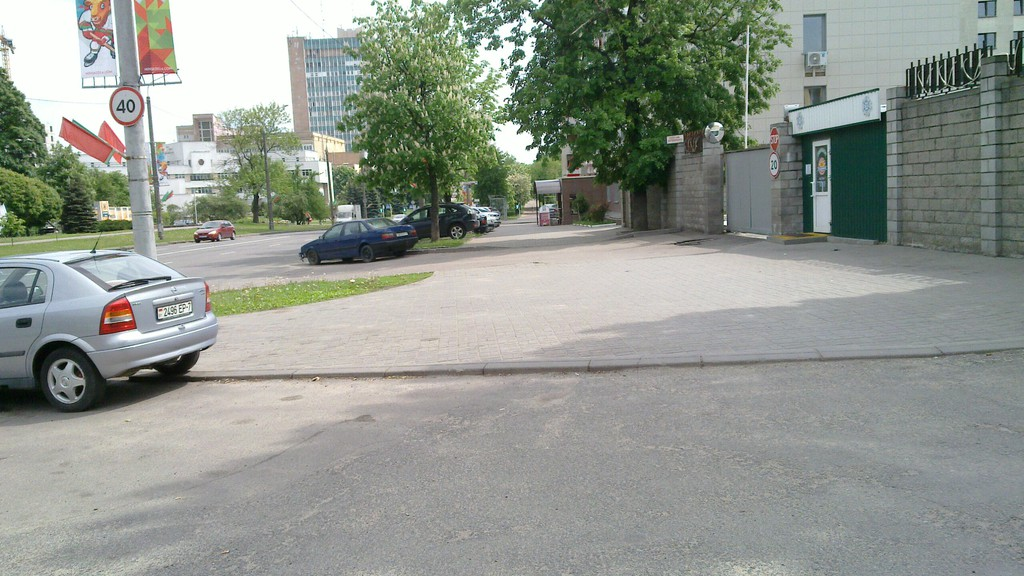
\includegraphics[width=\textwidth]{Pictures/1000000000000A00000005A0A3C4B935.jpg}
    \caption{Проезд к хладокомбинату}
\end{figure}

\begin{figure}[h!]
    \centering
    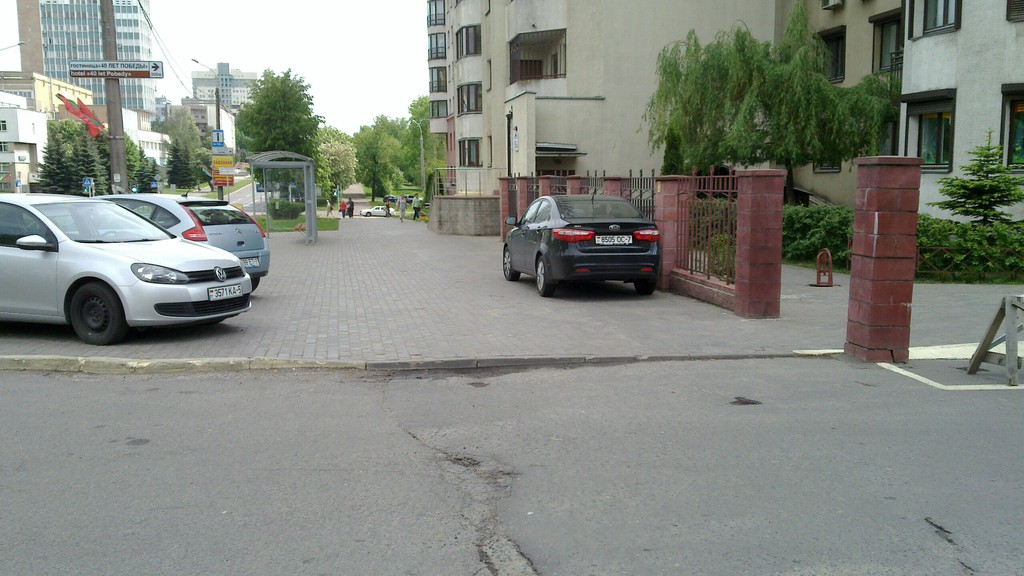
\includegraphics[width=\textwidth]{Pictures/1000000000000A00000005A08E05568F.jpg}
    \caption{Проезд к дому №50В}
\end{figure}

\begin{figure}[h!]
    \centering
    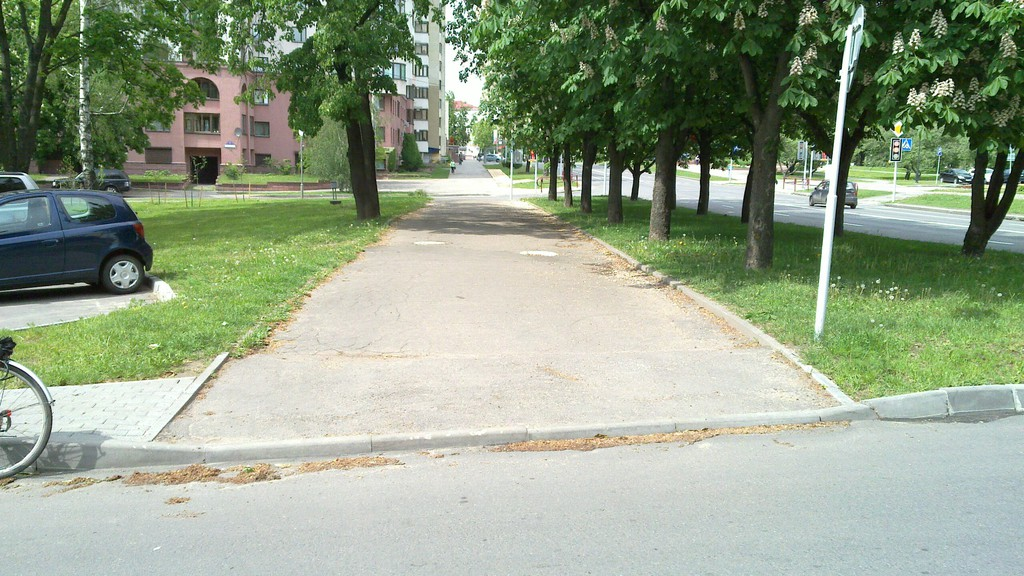
\includegraphics[width=\textwidth]{Pictures/1000000000000A00000005A0FA048808.jpg}
    \caption{Проезд к станции скорой помощи}
\end{figure}

\clearpage
\newpage

\subsection*{Октябрьский район}%
\emph{Участок}: Брилевская ул. и ул. Лейтенанта Кижеватова, от Аэродромной ул. до ул. Корженевского.

\emph{Понижение бортовых камней}:
Вместо понижения бортовых камней выполнено обустройство асфальтовых пандусов, многие из которых имеют угол наклона намного круче нормативного. Некоторые из обустроенных пандусов уже повреждены снегоуборочной техникой. На фото приведены только некоторые из таких объектов.

\emph{Разметка, знаки}: присутствуют частично, остались от старой велодорожки (проекту не соответствуют).

\emph{Заключение}: несмотря на заметное облегчение передвижения велосипедистов по маршруту, объект не готов: требуется понижение бортовых камней, установка знаков, нанесение разметки.

\begin{figure}[h!]
    \centering
    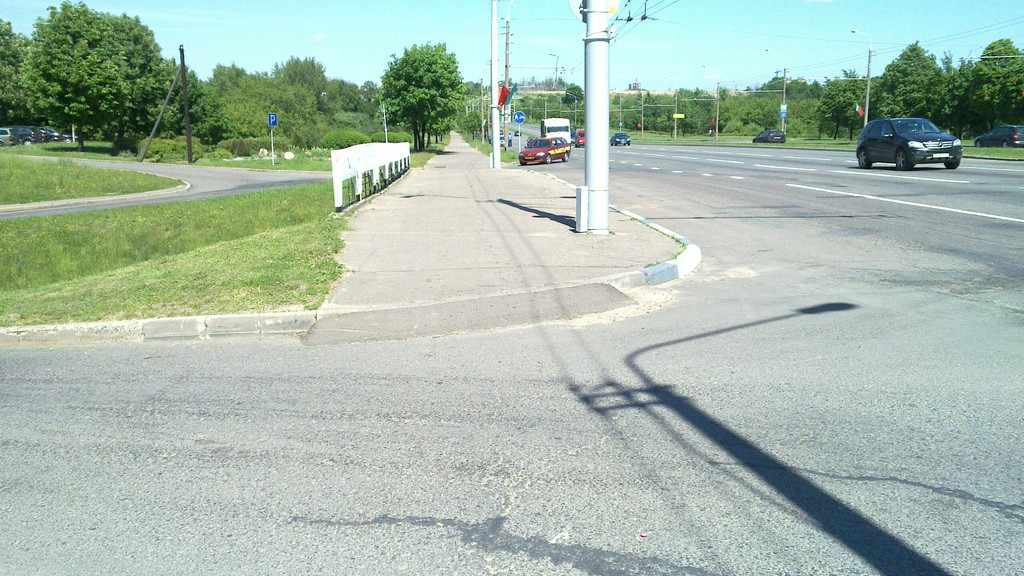
\includegraphics[width=\textwidth]{Pictures/1000000000000A00000005A0A7D8B156.jpg}
    \caption{Проезд к БСМП. Вместо понижения обустроен пандус, угол наклона пандуса больше нормативного}
\end{figure}

\begin{figure}[h!]
    \centering
    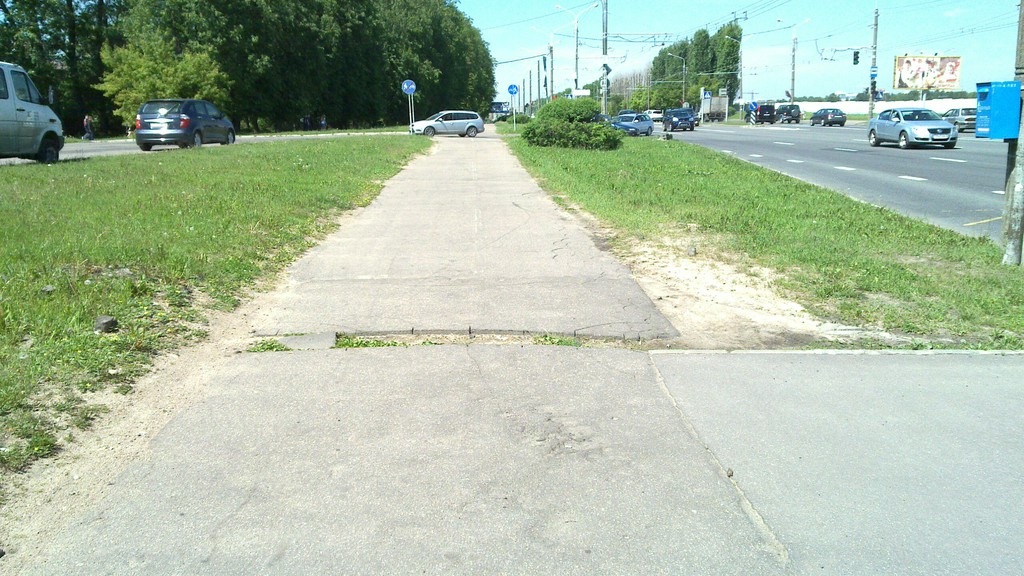
\includegraphics[width=\textwidth]{Pictures/1000000000000A00000005A0CF7F4A3C.jpg}
    \caption{Район остановки «Рижская». После монтажа рекламного щита не восстановлено асфальтовое покрытие}
\end{figure}

\begin{figure}[h!]
    \centering
    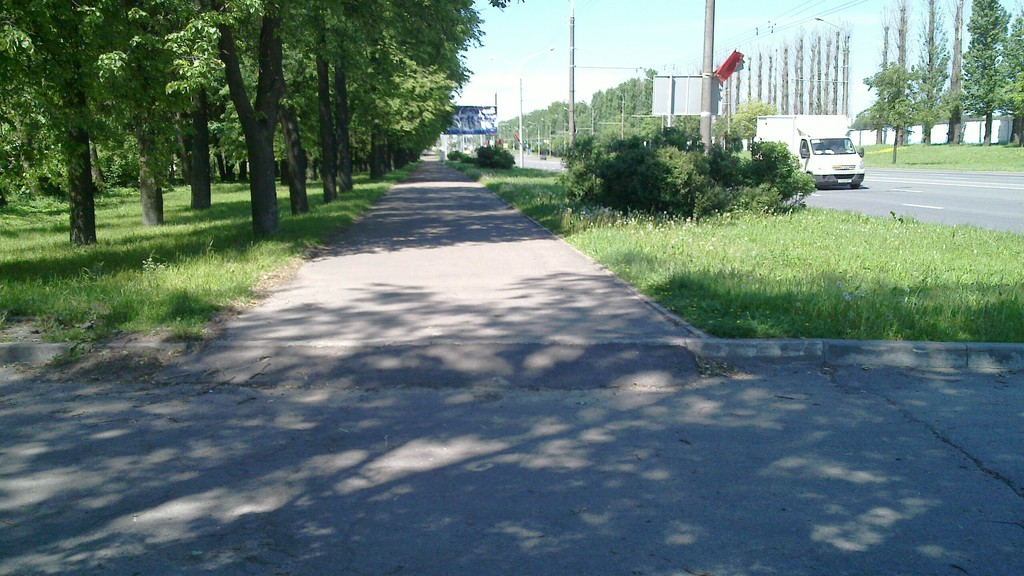
\includegraphics[width=\textwidth]{Pictures/1000000000000A00000005A003D7DB9F.jpg}
    \caption{Пандус вместо понижения. Угол наклона больше нормативного}
\end{figure}

\begin{figure}[h!]
    \centering
    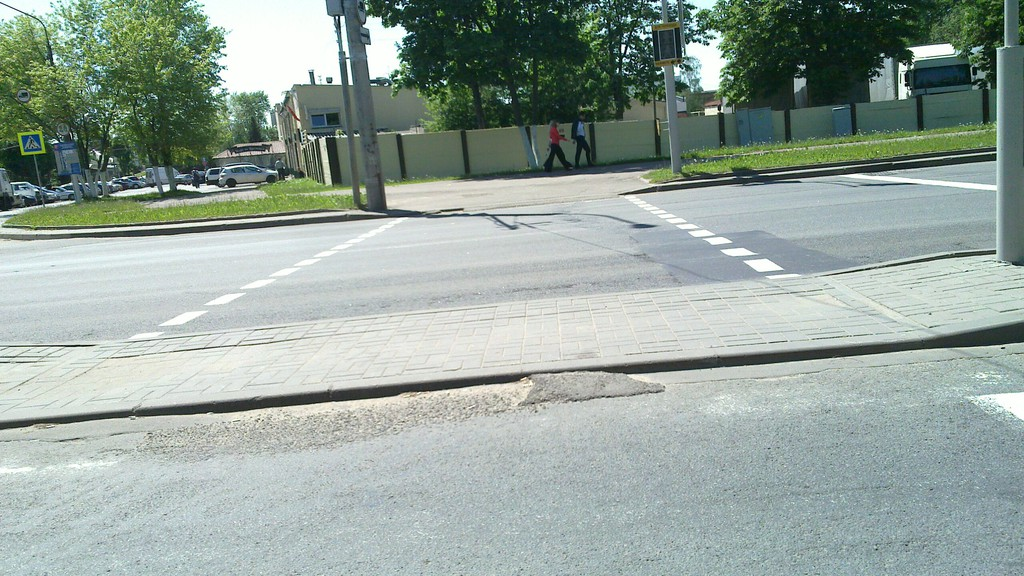
\includegraphics[width=\textwidth]{Pictures/1000000000000A00000005A06669A335.jpg}
    \caption{Переход через ул. Кижеватова в районе Брестской ул. Устроенный пандус повреждён}
\end{figure}

\clearpage
\newpage

\subsection*{Московскийрайон}%
\emph{Участок}: ул. Рафиева от ул. Алибегова до Слободской ул.

\emph{Понижение бортовых камней}:
Понижения бортовых камней выполнены в основном в соответствии с проектом, хотя в некоторых местах область понижения не доходит до границ тротуара (не соответствует типовой схеме понижения из проектной документации), на что следует обратить внимание в будущих проектах. Не выполнено понижение бортовых камней на перекрёстке с ул. Алибегова. При строительстве проезда к новому супермаркету (Рафиева, 56) были нарушены нормы безбарьерной среды.

\emph{Разметка, знаки}: отсутствуют

\emph{Заключение}: понижения бортов выполнены практически все, кроме перекрёстка Рафиева-Алибегова. Требуется исправление нарушений при строительстве проезда к супермаркету (Рафиева, 56), нанесение разметки, установка знаков. Объект не готов.

\begin{figure}[h!]
    \centering
    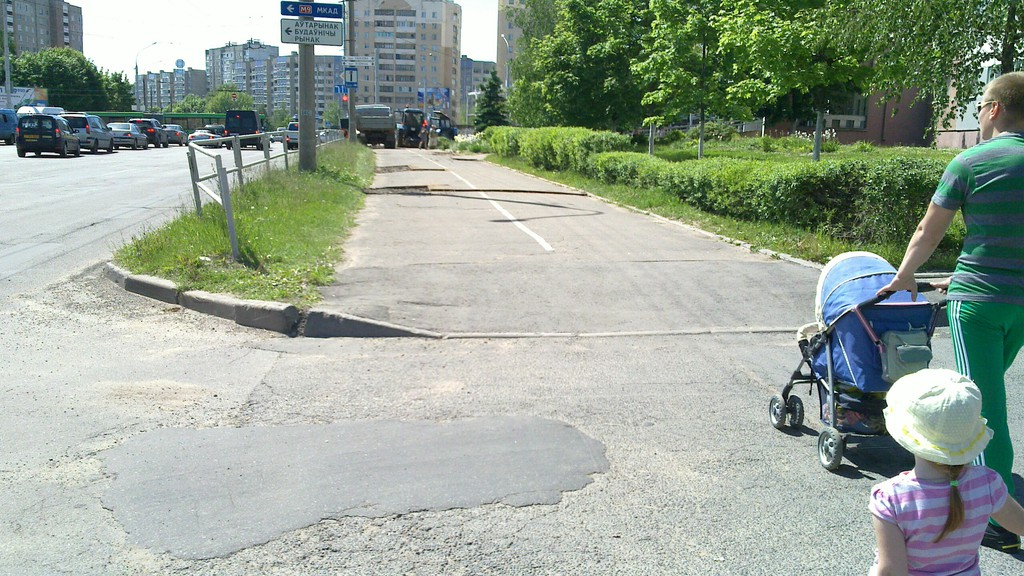
\includegraphics[width=\textwidth]{Pictures/1000000000000A00000005A0F05C02E6.jpg}
    \caption{Типичная ошибка: бортовой камень понижен, но зона понижения не доходит до края тротуара}
\end{figure}

\begin{figure}[h!]
    \centering
    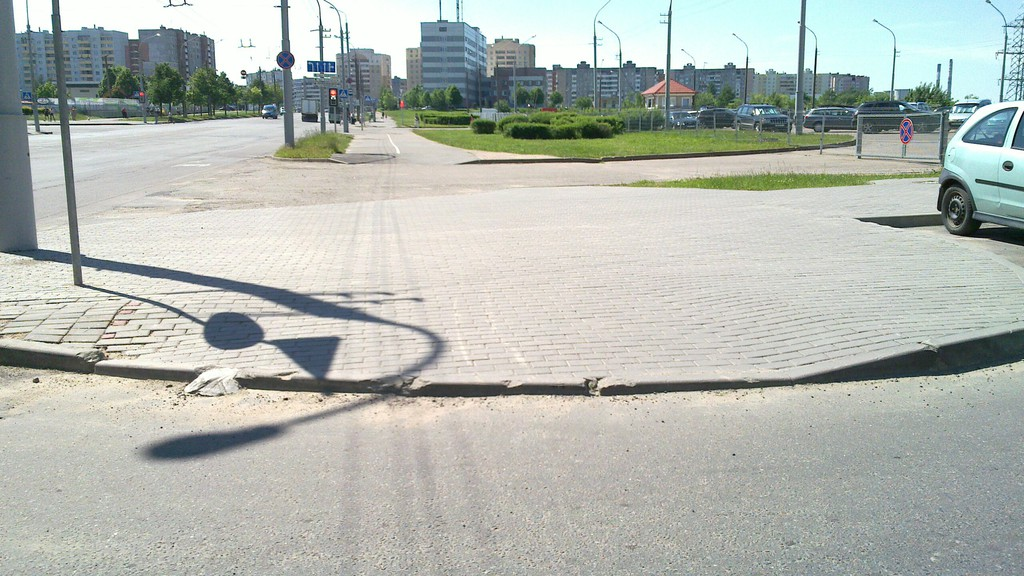
\includegraphics[width=\textwidth]{Pictures/1000000000000A00000005A0471C66C7.jpg}
    \caption{Высокий бордюр на проезде к супермаркету (Рафиева, 56). Виден мини-пандус, самостоятельно обустроенный для себя неким велосипедистом. Из-за ненормативной высоты бортовой камень уже повреждён техникой}
\end{figure}

\begin{figure}[h!]
    \centering
    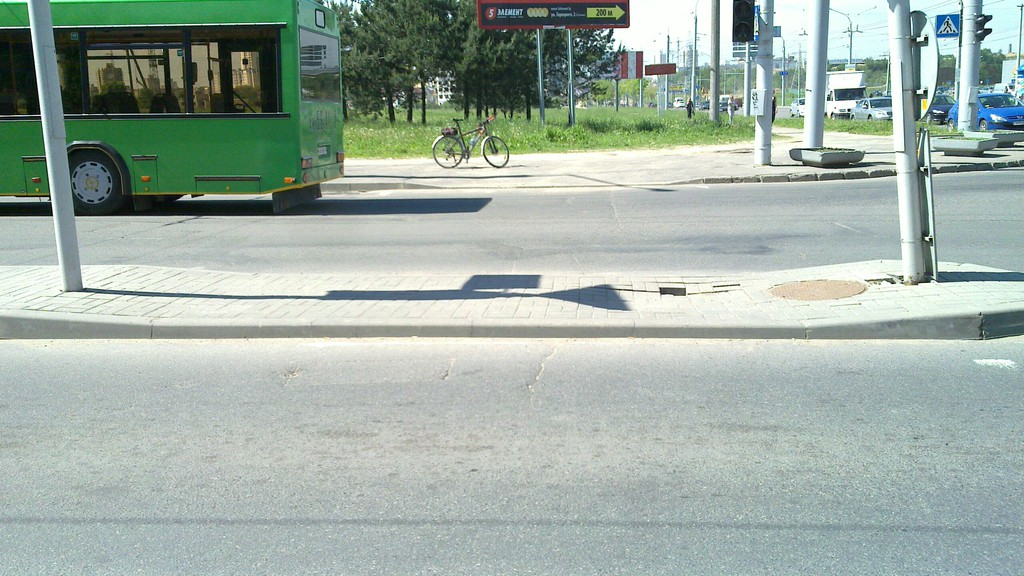
\includegraphics[width=\textwidth]{Pictures/1000000000000A00000005A075E04846.jpg}
    \caption{Перекрёсток Рафиева-Алибегова, переход через ул. Рафиева. При строительстве светофорного объекта нормы по высоте бордюров нарушены, в ходе выполнения проекта бортовой камень не понижен}
\end{figure}

\begin{figure}[h!]
    \centering
    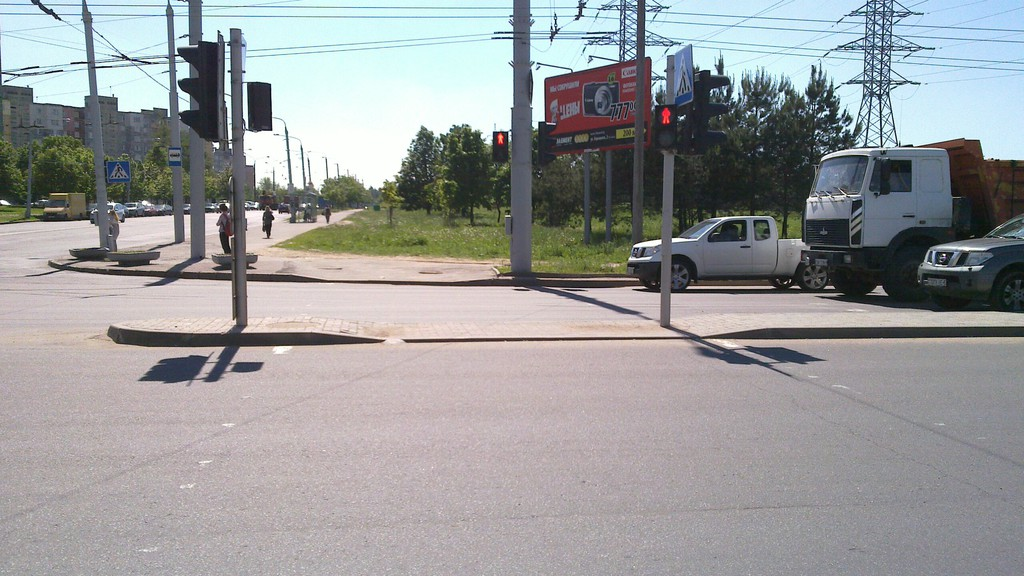
\includegraphics[width=\textwidth]{Pictures/1000000000000A00000005A0BE0179A9.jpg}
    \caption{Перекрёсток Рафиева-Алибегова, переход через Алибегова. Бортовые камни не понижены}
\end{figure}

\clearpage
\newpage

\subsection*{Ленинский район}%
\emph{Участок}: ул. Якубова от универсама «Свислочь» до ул. Малинина, ул. Малинина вдоль жилой застройки от ул. Якубова до канала Слепянской водной системы.

\emph{Понижение бортовых камней}:
Бортовые камни либо не понижались вовсе, либо устроены асфальтовые пандусы, угол наклона которых не соответствует нормативному. Некоторые из пандусов уже повреждены или уничтожены. Предусмотренные проектом малые архитектурные формы для ограничения заезда автомобилей на тротуары не установлены.

\emph{Разметка, знаки}: разметка нанесена частично

\emph{Заключение}: объект не готов.

\clearpage
\end{document}
